\chapter{Motivación e introducción}


\section{Sistemas basados en dispositivos FPGAs} 

Las FPGAs (\textit{Field Programmable Gate Arrays}), son dispositivos semiconductores basados en matrices de bloques lógicos configurables
(\textbf{CLB}) que están conectados mediante interconexiones programables \cite{fpga_xilinx}. 

Los \textbf{CLB} constan de celdas lógicas llamadas ``\textit{Slices}'', formadas por LUTs (\textit{tablas de consulta}), flip-flops y 
multiplexores de entrada y salida (Figura \ref{arqFPGA}). Una LUT almacena una lista de salidas lógicas para cualquier combinación de 
entradas. 

\begin{figure}[H]
    \centering
    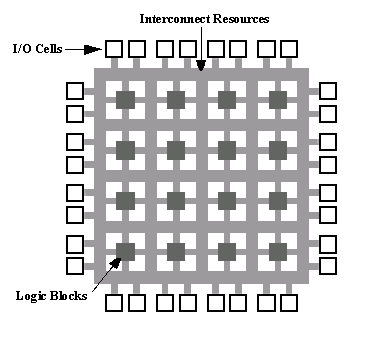
\includegraphics[width = 1\textwidth]{imagenes/arqFPGA.png}
    \caption{\textit{Arquitectura de una FPGA}}\label{arqFPGA}
\end{figure}

Estas FPGAs pueden ser reprogramadas para  algún trabajo específico o para cambiar los requisitos de funcionalidad después de su 
fabricación. Algunas pueden ser programadas una sola vez mientras que otras pueden ser reprogramadas una y otra vez. A estos 
dispositivos que son programados una única vez son referidos como \textbf{OTP} (\textit{one-time programmable}).

\textit{Field Programmable}, se refiere al hecho de que su programación se hace "\textit{en el campo}" a diferencia de otros dispositivos 
que su funcionalidad está programada por el fabricante \cite{maxfield1}.

Hay muchos tipos diferentes de circuitos integrados digitales, entre los que destacamos \textbf{PLDs} (\textit{Programmable Logic Devices}), 
\textbf{ASICs} (\textit{Application-Specific Integrated circuits}), \textbf{ASSPs} (\textit{Application-Specific Standard Parts}) y \textbf{FPGAs}.

Los \textbf{PLDs} son dispositivos con una arquitectura interna predeterminada por el fabricante, creados para ser configurados por 
ingenieros en el campo para realizar diferentes funciones. En comparación a las \textbf{FPGAs}, contiene un número limitado de puertas lógicas 
y las funciones que se suelen implementar son más pequeñas y simples.

Por otro lado los \textbf{ASICs} y los \textbf{ASSPs} contienen cientos de millones de puertas lógicas y se usan para crear grandes y complejas 
funciones. Ambos están basados en los mismos procesos de diseño y tecnologías y pueden ser usados por millones de usuarios y compañias. La 
única diferencia es que un \textbf{ASIC} está diseñado y fabricado para una aplicación en concreto, mientras que un \textbf{ASSP} lo está 
para un dominio de aplicaciones.

Así, las \textbf{FPGAs} se encuentran entre los \textbf{PLDs} y los \textbf{ASICs} porque su funcionalidad puede ser diseñada en el campo como 
los \textbf{PLDs}, pero pueden contener millones de puertas lógicas y ser usadas para implementar funciones complejas que previamente sólo 
podían ser realizadas usando \textbf{ASICs}. 

El coste de un diseño de \textbf{FPGA} es mucho menor que el de uno de un \textbf{ASIC}. Al mismo tiempo, los cambios de diseño implementados 
son más fáciles en \textbf{FPGAs} y el tiempo de comercialización es más rápido \cite{maxfield2}.

Las FPGAs \textbf{SoC}(\textit{System-on-chip}) tienen una gran capacidad de procesamiento para adaptarse a diferentes aplicaciones. Un SoC 
de bajo costo y consumo se puede enfocar en aplicaciones de gran volumen como tarjetas de procesamiento de vídeo o protocolo de puentes. Sin 
embargo, hay otros SoCs que se enfocan en aplicaciones de alto rendimiento en comunicaciones o computación de alto rendimiento.

A mediados del año 1980 llegaron las FPGAs, que eran usadas para implementar lógicas simples, máquinas de estados con una complejidad media 
y tareas de procesamiento de datos. A principios de los 90s, el mercado en el que se vendían se extendió al área de las telecomunicaciones 
debido a que el tamaño y sofisticación de las mismas empezaron a crecer. A finales de los 90s, el uso de las FPGAs en aplicaciones de consumo 
e industriales tuvo un enorme crecimiento.

Las FPGAs a menudo son utilizadas para crear prototipos de diseños ASIC o para tener un plataforma hardware donde verificar la implementación 
física de nuevos algoritmos \cite{maxfield1}. 

Actualmente se pueden encontrar FPGAs de alto rendimiento con millones de puertas. Algunos de estos dispositivos tienen núcleos de 
microprocesador integrados, dispositivos de entrada-salida de alta velocidad y similares. El resultado es que actualmente las FPGAs pueden ser 
usadas para implementar casi cualquier cosa en distintos ámbitos como por ejemplo:

\begin{itemize}
    \item \textbf{Aeroespacial y defensa} 
    \item \textbf{Emulación y Prototipado}
    \item \textbf{Audio} 
    \item \textbf{Automoción} 
    \item \textbf{Broadcast} 
    \item \textbf{Electrónica de consumo} 
    \item \textbf{Centro de procesamiento de datos} 
    \item \textbf{Computación de alto rendimiento} 
    \item \textbf{Industria} 
    \item \textbf{Medicina} 
    \item \textbf{Comunicaciones}
    \item \textbf{Inteligencia Artificial}
    \item \textbf{Procesamiento de imágenes}
    \item \textbf{Seguridad}
\end{itemize}

\section{Niveles de síntesis automática}  

Una de las características principales de un lenguaje de descripción hardware es que a partir de una descripción RTL se puede generar un 
circuito físico. La síntesis es el paso de un nivel de descripción a uno de nivel inferior.

La síntesis física consiste en la ubicación, es decir, decidir dónde colocar todos elementos lógicos, y en el enrutamiento, en el que se 
decide cómo se interconectan los elementos en la FPGA.

La síntesis RT-lógica es un proceso en el se crea un diseño RTL (\textit{Register-Transfer Level}), que es una abstracción del diseño 
en el que se modela el circuito digital, y luego esa representación RTL es convertida a una mezcla de registros y ecuaciones 
booleanas equivalentes. 

La principal diferencia entre síntesis RT y síntesis de alto nivel es que la primera parte de una descripción en la que de forma 
explícita se especifican las operaciones que deben realizarse en cada ciclo de reloj, mientras que la planificación de operaciones 
en ciclos de reloj se realiza de forma automática en la segunda.

La síntesis de alto nivel une hardware y software de manera que los diseñadores hardware pueden trabajar con un alto nivel de abstracción 
y los desarrolladores software pueden acelerar las pas partes computacionalmente complejas de sus algoritmos en una FPGA. 

El uso de una metodología de diseño de síntesis de alto nivel permite desarrollar algoritmos con respecto a la implementación ya que 
consume tiempo de desarrollo, validar el correcto funcionamiento de un diseño de forma más rápida que con lenguajes de descripción 
hardware tradicionales o crear implementaciones hardware de alto rendimiento

\section{Plataformas de desarrollo} 

Actualmente hay muchas empresas que fabrican FPGAs, pero en el top 5 se pueden encontrar \textit{Xilinx}, \textit{Altera}, 
\textit{Lattice Semiconductor}, \textit{Microsemi (antiguo Actel)} y \textit{QuickLogic}. Tanto Xilinx como Altera ocupan un 89\% 
del mercado, siendo Xilinx el líder desde hace muchos años. Xilinx tiene bastante variedad de FPGAs en cuanto a coste y rendimiento. 
Actualmente, la serie \textit{Virtex} y la serie \textit{Zynq-7000} de SoC ocupan el mercado de gama alta, la serie \textit{Kintex} 
de gama media y la serie \textit{Artix} de gama baja junto con la \textit{Spartan} que ha sido retirada del mercado.

La serie \textit{Virtex} integra lógica \textbf{FIFO} y \textbf{ECC}, bloques \textbf{Ethernet MAC}, bloques \textbf{DSP} (\textit{Procesador 
de señales digitales}), controladores \textbf{PCI-Express}. Además incluye hardware embebido con una función fija para funciones que se 
usan comúnmente como multiplicadores o memoria. 

La serie \textit{Kintex} se caracteriza por consumir menos energía que la serie anterior, incluyendo alto rendimiento y elementos necesarios 
para aplicaciones que tengan mucho volumen.

La serie \textit{Artix} se basa en la arquitectura unificada de la serie \textit{Virtex}. Esta serie está diseñada para aplicaciones con 
rendimiento de bajo consumo. 

Dependendiendo de la síntesis que queramos realizar podemos encontrar distintos software:

\begin{itemize}
    \item \textbf{Herramientas de síntesis RT-lógica}:
        \begin{itemize}
            \item \textit{Synplify Pro}, \textit{Synplify Premier} (\textit{Synopsis})
            \item \textit{Precision RTL Plus}, \textit{LeonardoSpectrum} (\textit{Mentor Graphics})
            \item \textit{Quartus} (\textit{Altera})
            \item \textit{Vivado} (\textit{Xilinx})
        \end{itemize}
    \item \textbf{Herramientas de síntesis de alto nivel}:
        \begin{itemize}
            \item \textit{Synphony C Compiler} (\textit{Synphony})
            \item \textit{Impulse coDeveloper} (\textit{Impulse C})
            \item \textit{Vivado High Level Synthesis} (\textit{Xilinx})
            \item \textit{SDSoc} (\textit{Xilinx})
            \item \textit{SDAccel} (\textit{Xilinx})
            \item \textit{Intel SDK for OpenCL} (\textit{Intel Altera})
            \item \textit{Intel HLS Compiler} (\textit{Intel Altera})
        \end{itemize}
\end{itemize}

La última herramienta comercializada por Xilinx, \textit{Vitis} es un entorno de desarrollo de aplicaciones que sustituye a las herramientas 
\textit{SDSoc} y \textit{SDAccel} que permite utilizar tanto FPGAs en tarjetas aceleradoras on premise y en la nube, como FPGAs con procesadores 
empotrados. Incorpora una herramienta de síntesis de alto nivel (\textbf{Vitis HLS}) que pretende reducir las diferencias entre escribir 
funciones para su ejecución software o para su implementación hardware. Y se dispone incluso de bibliotecas con funciones prediseñadas 
para diferentes dominios de aplicación (inteligencia artificial, visión, etc.).

Las plataformas de desarrollo con propósito académico que comercializa Xilinx son \cite{students}:

\begin{itemize}
    \item \textbf{7-series} - \textit{Spartan-7}, \textit{Artix-7}, \textit{Kintex-7}, \textit{Virtex-7}
    \item \textbf{Zynq} - \textit{ZYBO}, \textit{ZYBO Z7}, \textit{ZedBoard}
    \item \textbf{Spartan} - \textit{Spartan-6}, \textit{Spartan-3E}
    \item \textbf{Virtex} - \textit{Virtex-6}, \textit{Virtex-5}, \textit{Virtex-4}, \textit{Virtex-2P}
\end{itemize}


\section{Estructura de la memoria} 
 
 
 